\section{WGAN-GP}
To create a \gls{WGAN-GP} the architecture of the \gls{WGAN} can be modified to remove the weight clipping constraints from the critic, and it's loss can be changed to have a gradient penalty term as described in \autoref{sub:wgan_gp}. The gradient penalty should offer a better alternative to weight clipping and in turn produce better results.

\subsection{MNIST}
Training the \gls{WGAN-GP} on the \gls{MNIST} dataset produced the results seen in \autoref{fig:wgan_gp_mnist_metrics}. Observe how the overall value of the metrics has improved significantly when compared to the \gls{WGAN} approach.
\begin{figure}[hbt]
    \centering
    \caption{Metrics when training a WGAN-GP on MNIST}
    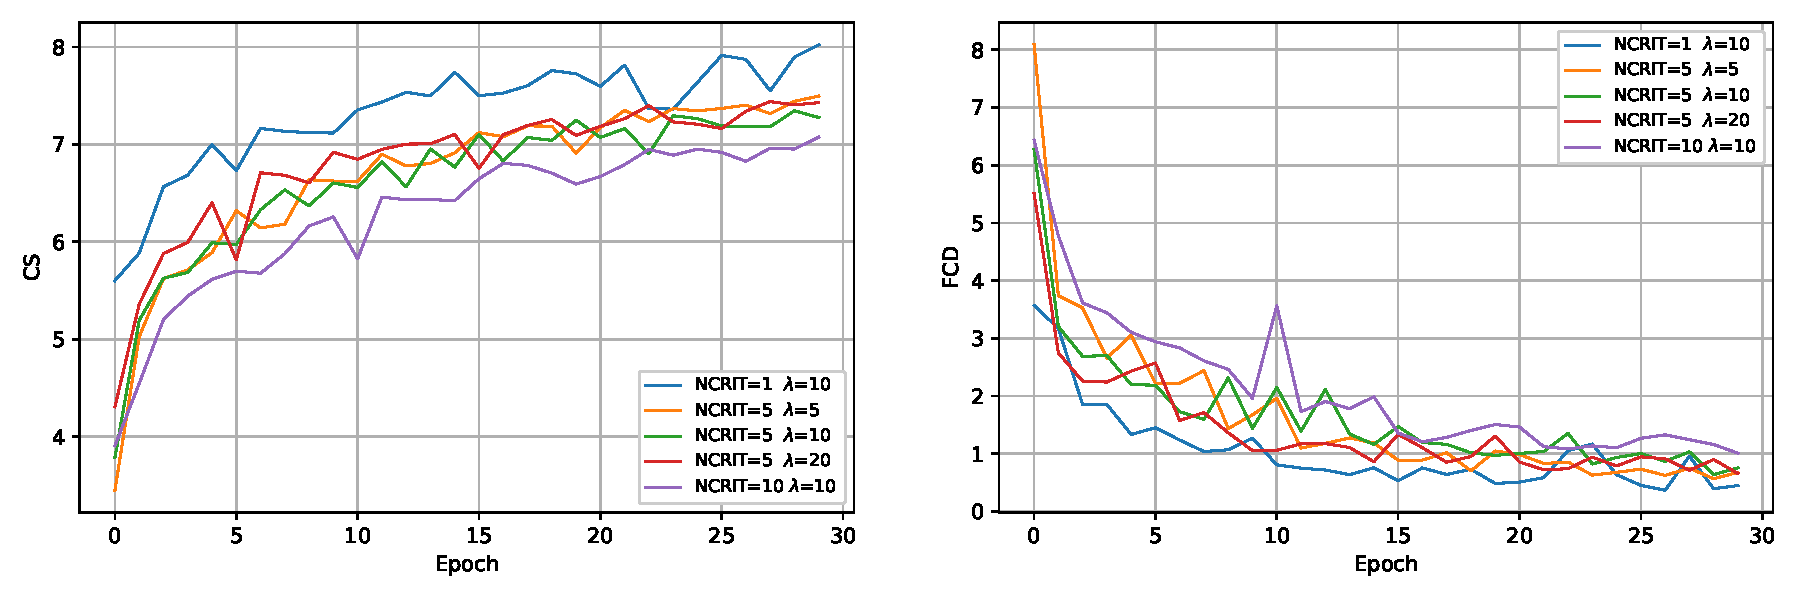
\includegraphics[width=\textwidth]{chapters/Experiments/WGAN-GP/mnist_metrics.pdf}
    \fonte{From the author (2021)}
    \label{fig:wgan_gp_mnist_metrics}
\end{figure}

The same behaviour related to the number of iterations for the critic can be seen, that is, more critic iterations tend to perform less well. The \gls{lambda} term, which regulates the strength of the gradient penalty, seems to produce similar results for all values tested. Contrary to the case seen for the \gls{WGAN}, this actually agrees with the recommended value of 10 given by the authors of the \gls{WGAN-GP} paper \cite{wgan-gp2017}.

The samples produced by the overall best model (NCRIT=1  $\lambda$=10) are shown in \autoref{fig:wgan_gp_mnist_samples}.
\begin{figure}
    \centering
    \caption{Samples when training a WGAN-GP on MNIST}
    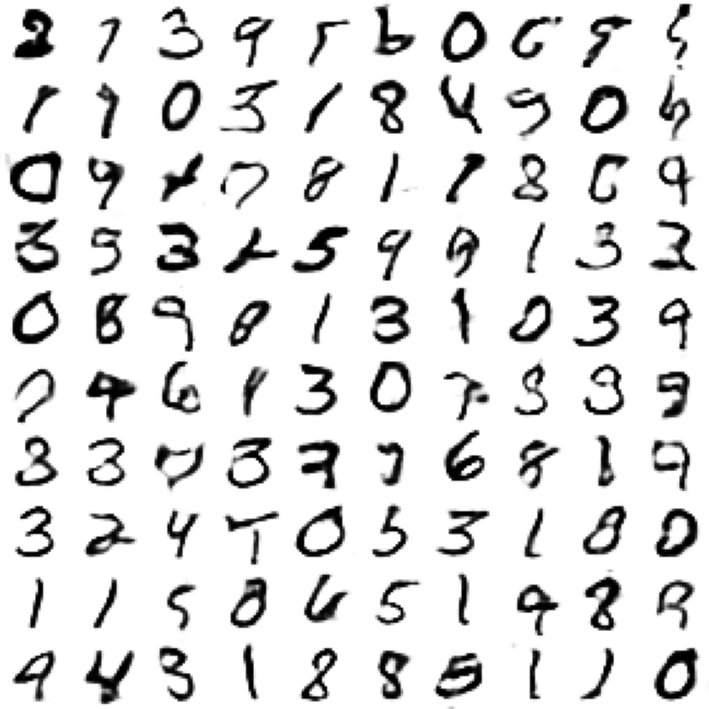
\includegraphics[width=0.6\textwidth]{chapters/Experiments/WGAN-GP/mnist_samples.png}
    \fonte{From the author (2021)}
    \label{fig:wgan_gp_mnist_samples}
\end{figure}


\subsection{Fashion MNIST}
Training the \gls{WGAN-GP} on the Fashion MNIST dataset produced the results seen in \autoref{fig:wgan_gp_fashion_metrics}. This gives very similar results and the same conclusions that were seen for the \gls{MNIST} experiments. \autoref{fig:wgan_gp_fashion_samples} shows the samples produced by the best model (\texttt{NCRIT=1 $\mathrm{\lambda}$=5}).
\begin{figure}[hbt]
    \centering
    \caption{Metrics when training a WGAN-GP on Fashion MNIST}
    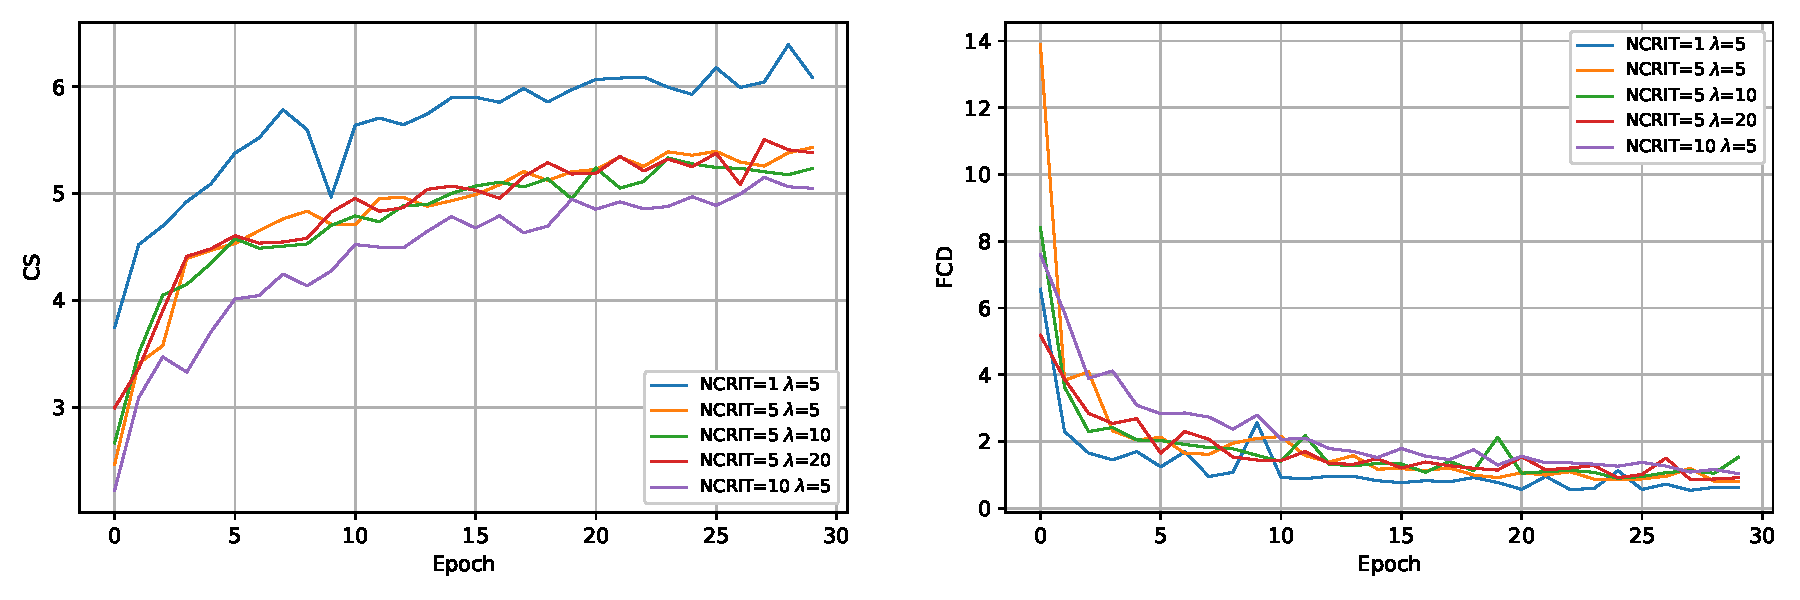
\includegraphics[width=\textwidth]{chapters/Experiments/WGAN-GP/fashion_metrics.pdf}
    \fonte{From the author (2021)}
    \label{fig:wgan_gp_fashion_metrics}
\end{figure}

\begin{figure}
    \centering
    \caption{Samples when training a WGAN-GP on Fashion MNIST}
    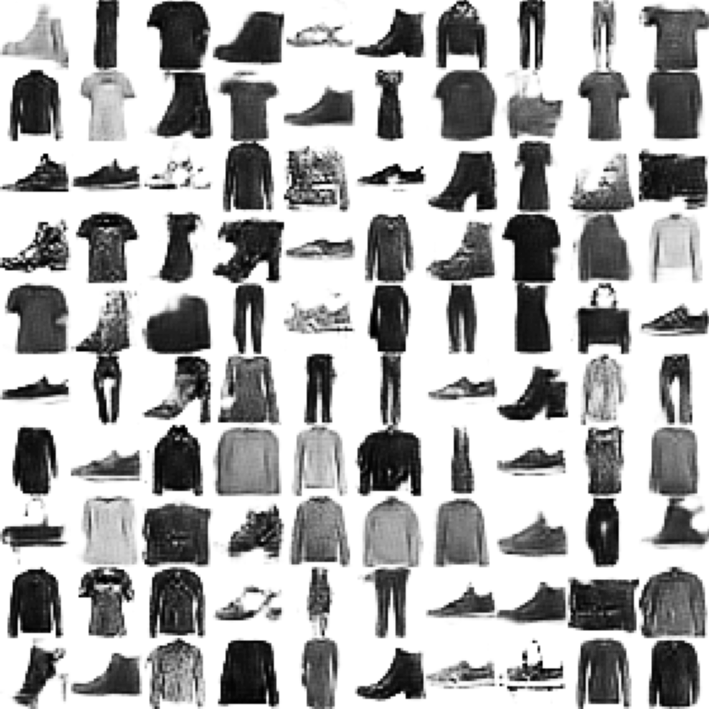
\includegraphics[width=0.6\textwidth]{chapters/Experiments/WGAN-GP/fashion_samples.png}
    \fonte{From the author (2021)}
    \label{fig:wgan_gp_fashion_samples}
\end{figure}


\subsection{CIFAR-10}
For these experiments it was used a value of 10 for \gls{lambda} since it followed the recommendation of the original authors and has also proved to work well in all cases tested. Training the \gls{WGAN-GP} on the \gls{CIFAR}-10 dataset produced the results seen in \autoref{fig:wgan_gp_cifar_metrics}.

Once again \gls{CIFAR}-10 proves itself considerably harder to train, these results show a higher degree of instability and also produced significant less favorable results when compared to \gls{DCGAN} and \gls{CGAN}, except for the case which used \texttt{NCRIT=1}. This still agrees with the previous results and shows how consistent this technique is, making hyperparameter search easier.

\begin{figure}[hbt]
    \centering
    \caption{Metrics when training a WGAN-GP on CIFAR-10}
    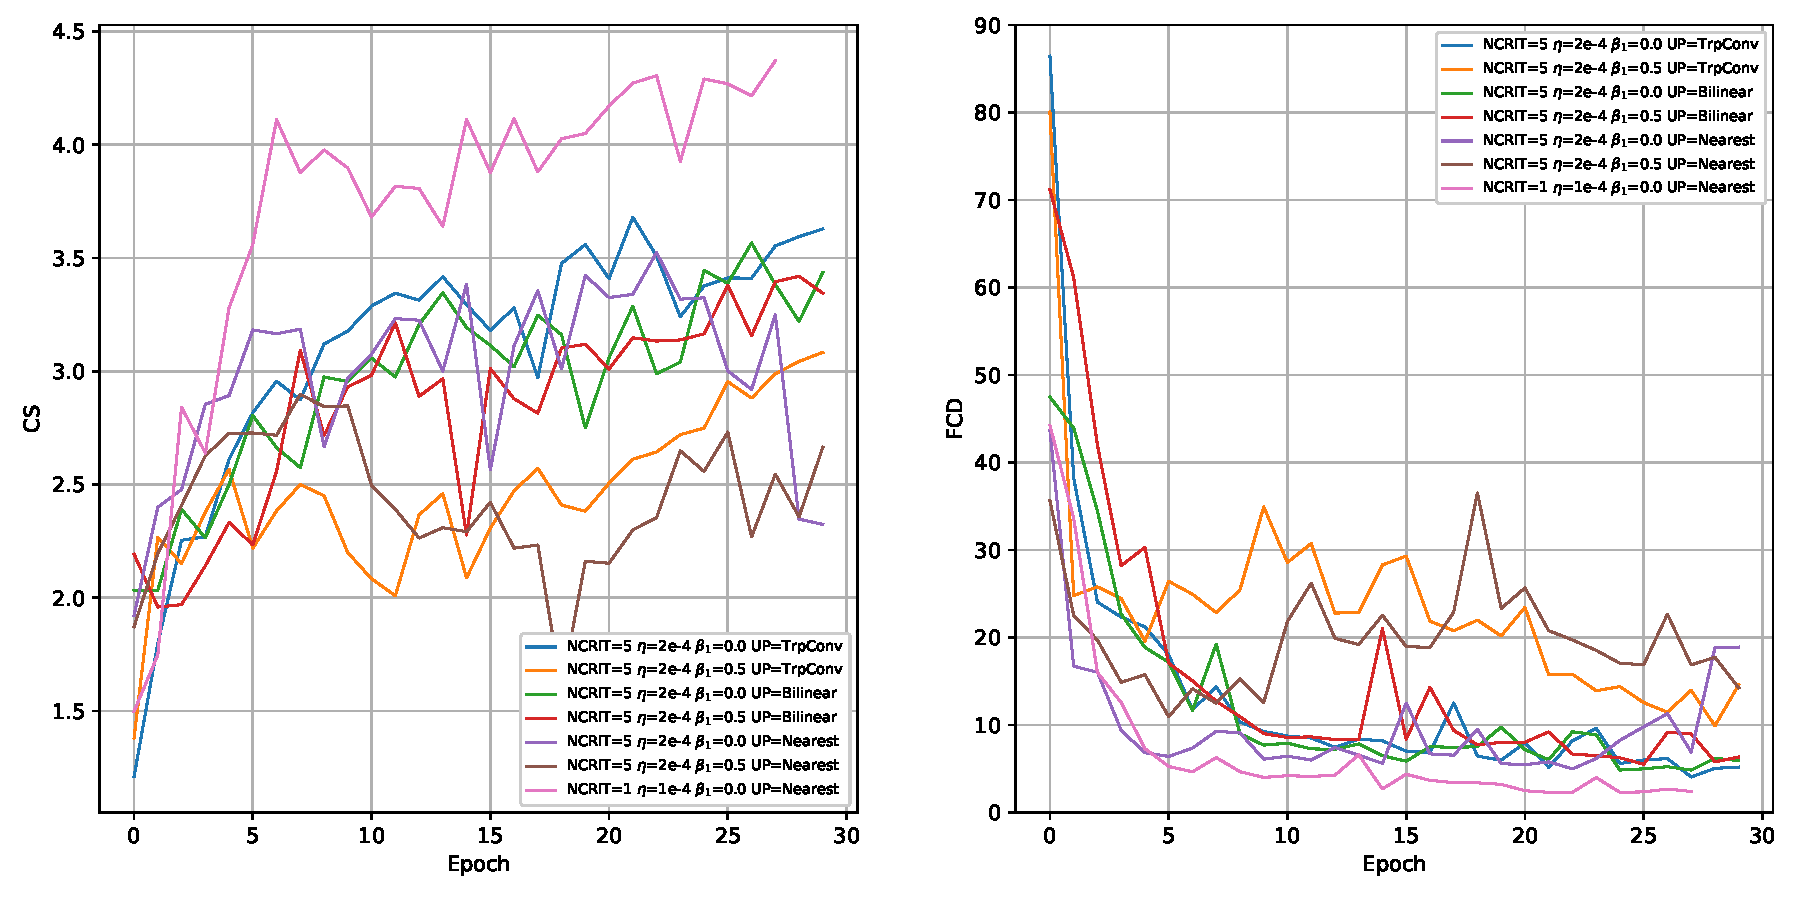
\includegraphics[width=\textwidth]{chapters/Experiments/WGAN-GP/cifar_metrics.pdf}
    \fonte{From the author (2021)}
    \label{fig:wgan_gp_cifar_metrics}
\end{figure}

The best resulting model (\texttt{NCRIT=1 $\eta$=1e-4 $\beta_1$=0.0 UP=Nearest}) was able to produce the samples shown in \autoref{fig:wgan_gp_cifar_samples}.
\begin{figure}
    \centering
    \caption{Samples when training a WGAN-GP on CIFAR-10}
    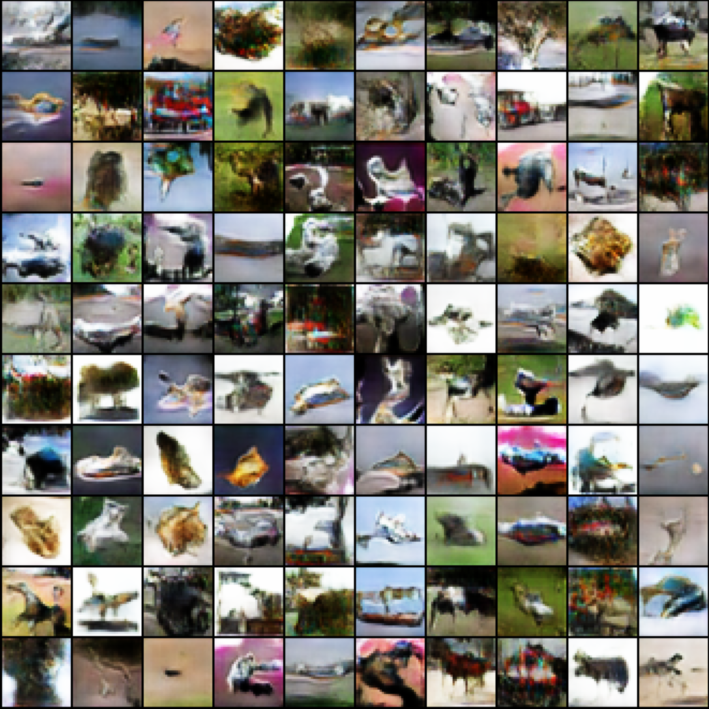
\includegraphics[width=0.5\textwidth]{chapters/Experiments/WGAN-GP/cifar_samples.png}
    \fonte{From the author (2021)}
    \label{fig:wgan_gp_cifar_samples}
\end{figure}
